In this chapter we provide a summary of our work on scalable graph similarity calculation
and concept discovery.
We describe the problem and some related work in Section \ref{sec:concepts-background}
and present our approach in Section \ref{sec:concepts-method}. We give our
findings in Section \ref{sec:concepts-main-findings} where we also present an experiment that was not part of our original work, that
bridges deep learning with out work to extract visual concepts from images.
We close the chapter with a discussion relating this work to our overall
research question in Section \ref{sec:concepts-discussion}

\section{Background}

\label{sec:concepts-background}

This work tackles the general problem of determining the similarity between \emph{objects}
in a data set, which can take the forms of cosine similarity between
items embedded in a low-dimensional representation \cite{word2vec}, or, as done
in this work, by modeling the problem as graph vertex similarity calculation.
We use the generic term \emph{object} to emphasize the generality of our
approach, made possible by the graph representation. In the paper we present examples from the linguistic,
music, and molecular biology domains, and in this dissertation provide an additional example using
generated image tags as input, in Section \ref{sec:concepts-openimages}.

In our approach we model the objects as nodes in graph and their interactions as edges,
initially weighted by a simple measure of correlation between the objects. In text for example, the
nodes would be words and the edges could be weighted by their mutual information \cite{mutual-information-nlp}.

The computation of all-to-all similarities in a graph can quickly become
intractable for large graphs. The popular SimRank algorithm developed by
\citet{simrank} for this purpose,
has a cubic time complexity with respect to the number of nodes in the graph.
Clearly then for large-scale graphs some form of approximation needs to be used
to make the computation feasible.


\section{Scalable Vertex Similarity and Concept Discovery}

\label{sec:concepts-method}

We deal with the scalability problem by using a two-step process to calculate similarities.
We first create a \emph{correlation graph} that models simple correlations between objects.
These correlations are easy to extract and do not necessarily hold semantic information.
For example,
given a corpus of text we can use a
co-occurence measure, like mutual information, between any two pairs of
words and use that as the edge weight between the two in the correlation graph.
We then compute the similarities between nodes by applying a transformation on this graph, to produce a graph which surfaces deeper,
semantic interactions which we term the \emph{similarity graph}.
In order to determine the similarity between objects in graph, we examine
their agreement in correlations to other objects: if two nodes are highly
correlated to similar sets of nodes, they are more likely to be similar themselves.

However, computing these all-to-all similarities can be challenging for massive
correlation graphs.
As in other works in this thesis, we apply a combination of using approximations to limit
the computational cost of the method, and develop a distributed algorithm that allows
us to scale-out learning and take advantage of modern computing clusters.

The first approximation we employ makes use of a characteristic that many real-world datasets exhibit,
that is, there exists a long-tail distribution of interactions between the items in a graph. These type
of ``small-world'' graphs, appear in areas like gene co-expression \cite{gene-small-world}, semantic networks \cite{semantic-small-world},
word co-occurrences \cite{words-small-world} and social networks (see \cite{barabasi-small-world} for further
examples).
This allows us to prune the input correlation graph significantly before transforming it,
while maintaining a controllable and small approximation error.

The second approximation has to do with the locality of the computation. Instead of trying
to solve the computationally intractable all-to-all similarity problem, we instead only look at
nodes that are one hop apart, keeping the computation local and dramatically computation cost per node in the graph.
This approximation is what makes the distributed implementation of the algorithm efficient.
In order to compute, for each pair of nodes in a neighborhood, their common sets of correlated nodes,
we need only examine the common sets of incoming edges per node. By distributing our graph
using the id of the incoming nodes as a key we can perform this computation using a
self-join operation, which involves no communication of data in the cluster. As a result
we are able to scale the computation to massive datasets, as we demonstrate by training on the
Google Books n-gram dataset, which corresponds to approximately 4\% of all the books ever
printed \cite{ngrams} (24.5 billion rows), in a few minutes.

Once we have built the similarity graph, we can go one step further in order to extract
groups of inter-similar objects that we call \emph{concepts}. These correspond to groups
of objects that belong to the same semantic group, based on their appearances in the context
of other objects. In the language example these could be words that describe the same
concept such as ``cities'', or words with the same syntactic and semantic purpose, like
groups of adverbs. To create these groups we apply a community detection method on top
of the similarity graph. Because the similarity graph itself can be large, we develop
a scalable approach which is based on the speaker-listener label propagation algorithm
(SLPA) \cite{slpa}. \todo{Do we explain community detection and label propagation here? Do we need to
include it in the BG?}

\section{Main Findings}

\label{sec:concepts-main-findings}

In the paper we provide examples of the output produced by the algorithm, and
perform a quantitative evaluation of the similarities produced using a gold standard dataset,
WordSim-353~\cite{wordsim}. Here we provide a summary of some of the experiments
presented in the paper, and a new set of results using images as input.

\subsection{Billion words corpus}

In the paper we perform an evaluation on the Billion word corpus~\cite{billion-word}
which contains approximately one billion tokens and was scraped from online news
sources. We create the correlation graph by using the relative co-occurrence frequency
of word pairs, that is the (directed) correlation between the words $i$ and $j$, $\rho_{i, j}$,
will be $c_{i,j}/c_i$ where $c_{i,j}$ the number of times the words co-occur within
a window, and $c_i$ the frequency of word $i$ in the corpus. For this experiment we
select a window size of two, meaning we only take into account bigrams.
We can see some example concepts uncovered by the algorithm in Figure \ref{fig:concepts-billion}.

\begin{figure}
	\centering
	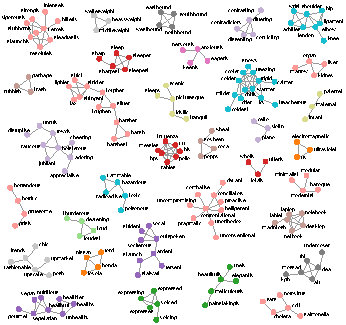
\includegraphics[width=\textwidth]{billion-words-example}
	\caption{Example concepts extracted from the Billion word corpus}
	\label{fig:concepts-billion}
\end{figure}

\subsection{Music}

We also perform experiments on a music listening dataset created by Celma from
the Last.fm music service~\cite{celma-long-tail}. The dataset contains 19 million
track plays from 992 users, which we use to create a correlation graph between
artists. The correlation measure $\rho_{i, j}$ is the number of times artist $i$ was followed
by artist $j$, divided by the total number of plays for artist $i$. Some example
artist concepts which correspond to music genres can be seen in Figure
\ref{fig:concepts-artists}.

\begin{figure}
	\centering
	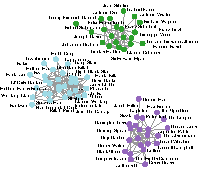
\includegraphics[width=0.8\textwidth]{artist-example}
	\caption{Example concepts extracted from the music listening dataset.}
	\label{fig:concepts-artists}
\end{figure}

\subsection{Uncovering Visual Concepts}

\label{sec:concepts-openimages}

In this experiment we make use of a combination of deep neural networks and our
algorithm to uncover visual concepts from images. Deep neural networks
can be trained on labeled datasets of images to recognize multiple objects
in an image \cite{deep-learning}. The networks' accuracy creates a unique opportunity
to generate visual concepts out of raw images: A network trained on labeled dataset
like ImageNet \cite{imagenet} can be used to generate labels from unlabeled raw images thus generating
a ``silver-standard'' dataset which we can use as input for our algorithm.

In our experiments we have used the OpenImages dataset \cite{openimages} which uses
multiple image classifiers to annotate images with labels from 19,794 different
classes. The complete training
dataset contains 9,011,219 images scraped from the Flickr service\footnote{\url{www.flickr.com}}, of complex scenes annotated with 8.4 objects per image on average.

We use the OpenImages data to create a correlation graph of objects: We form
a clique for every object that exists together in one image, creating a graph that represents
how objects commonly appear together in real images. Take for example the annotated
image shown in Figure \ref{fig:horse-hat}. The image is annotated with both the
\emph{horse} and \emph{cowboy hat} labels. All the labels in the image will form
a clique in our graph. Looking at another image, \ref{fig:hat-guitar} we can now
extend this graph, by connecting the \emph{cowboy hat} label with the \emph{guitar}
label, creating a second degree link between the \emph{horse} and \emph{guitar} labels.
By incorporating all such images, our correlation graph will have a representation of objects
that tend to appear together in the real world. Using this graph as input, we can apply our similarity
transformation to group together objects that belong to semantically similar classes
based on the similarity between the contexts in which they appear in, in the real world.
Finally we can apply our community detection algorithm to group together items to form
visual concepts in the similarity graph.

To illustrate the uncovered concepts, we take the 30,000 most similar
pair-wise object similarities and present the output similarity graph in Figure \ref{fig:openimages-concepts}, where the colors indicate the uncovered concepts.
To ease presentation we provide two zoomed-in parts in Figure \ref{fig:openimage-zoom},
where we can see objects that can roughly be described as ``uniformed people'' are grouped
together in Figure \ref{fig:openimages-military}, and objects that relate to cameras
grouped together in Figure \ref{fig:openimages-cameras}.

Using our algorithm in combination with deep learning models, we can use the wealth of unlabeled
images that exist in services like Flickr to create visual concepts.

\begin{figure}
	\centering
	\begin{subfigure}{\textwidth}
		\centering
		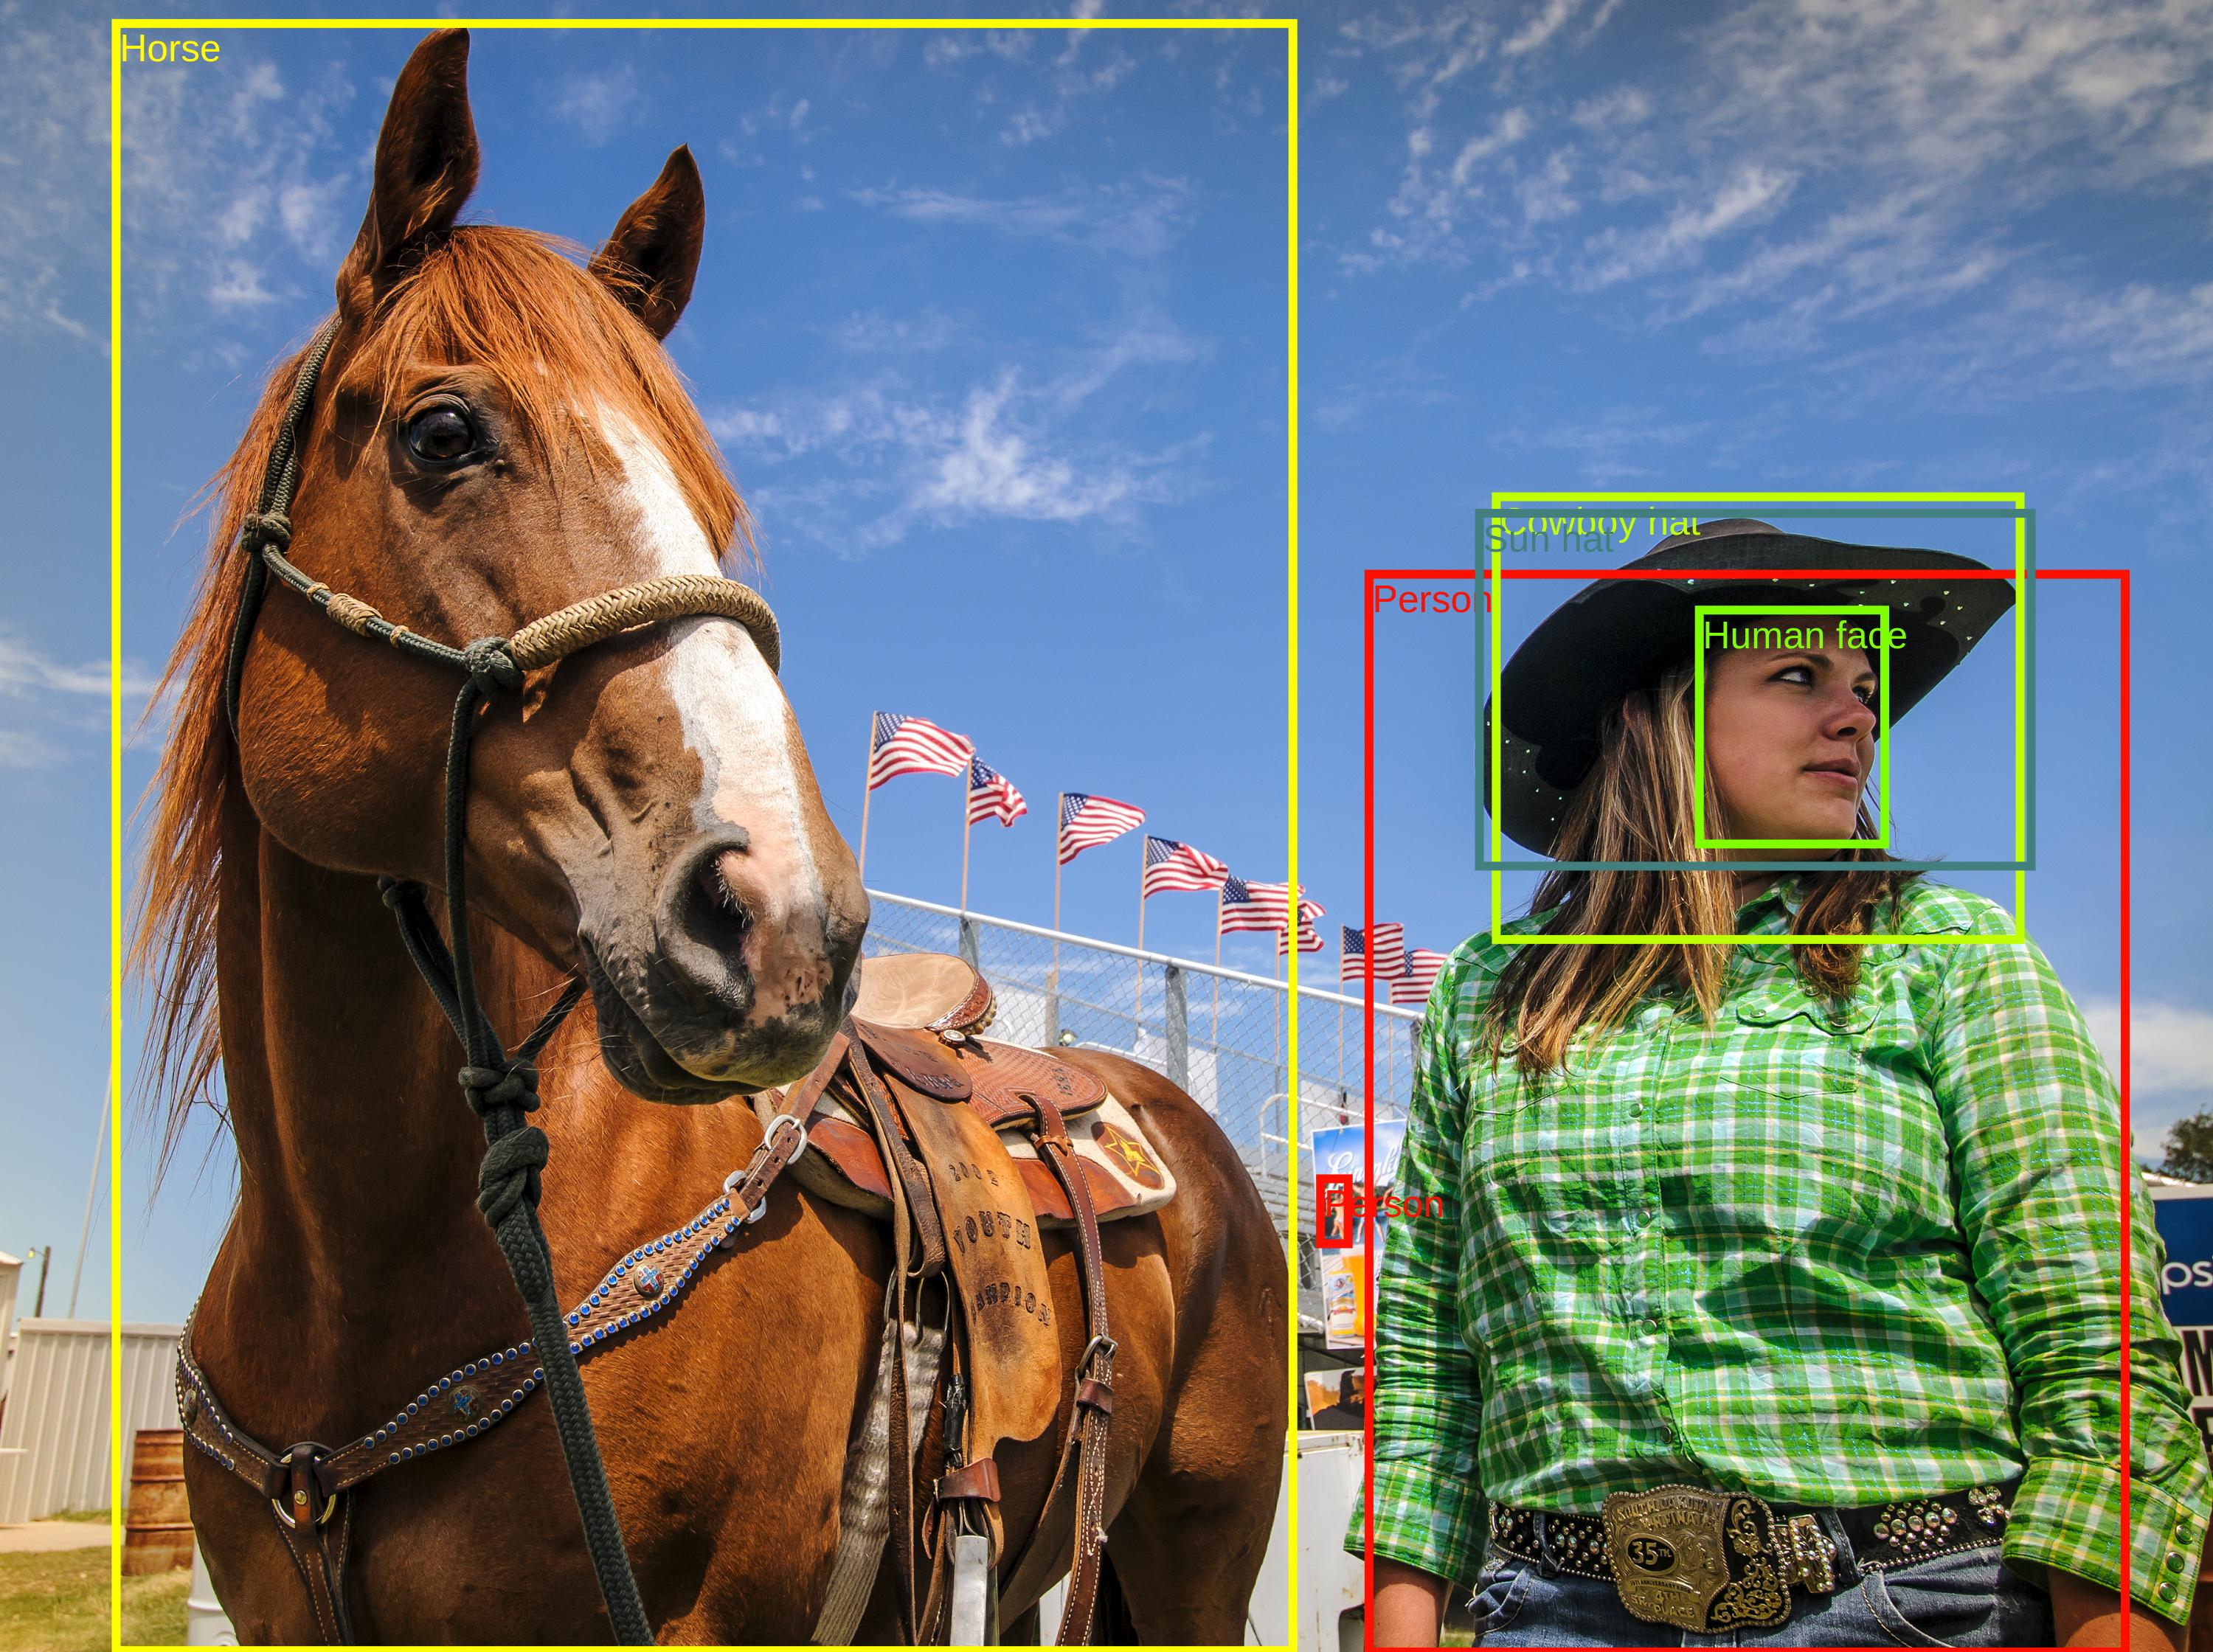
\includegraphics[width=0.9\textwidth]{horse-hat}
		\caption{An image that contains a horse and a cowboy hat.}
		\label{fig:horse-hat}
	\end{subfigure}
	~ %add desired spacing between images, e. g. ~, \quad, \qquad, \hfill etc.
	%(or a blank line to force the subfigure onto a new line)
	\begin{subfigure}{\textwidth}
		\centering
		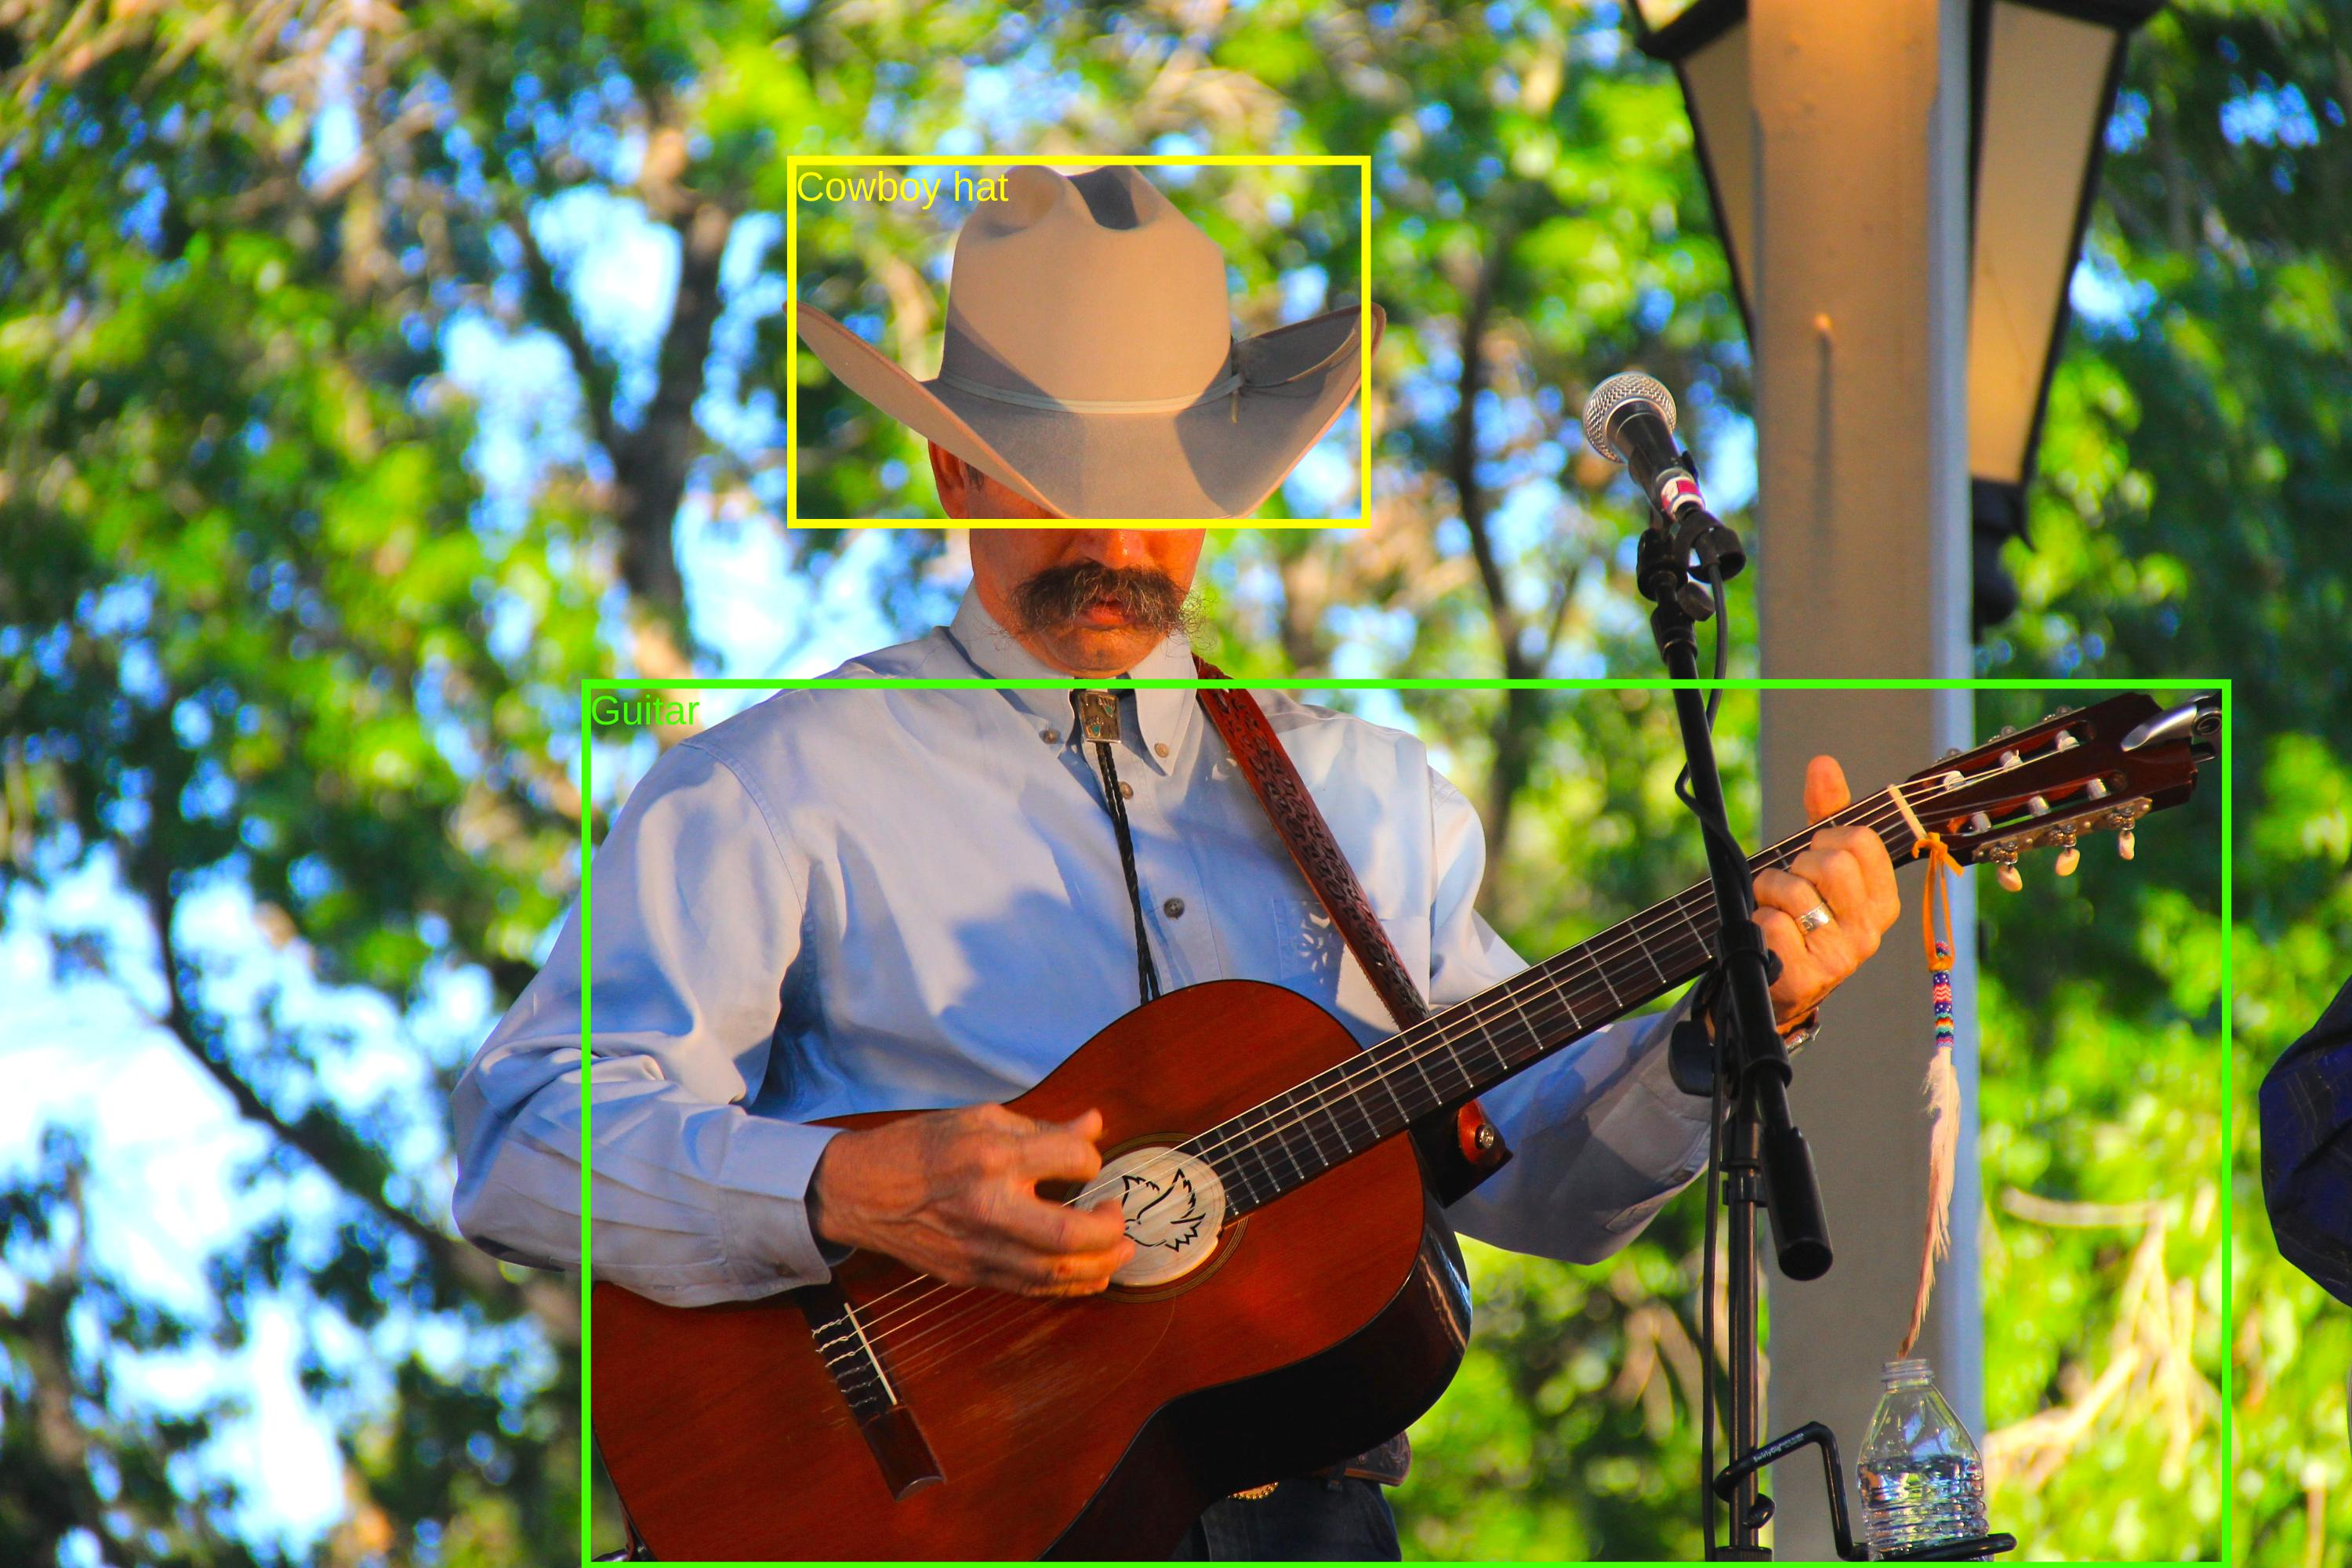
\includegraphics[width=0.9\textwidth]{hat-guitar}
		\caption{An image that contains a cowboy hat and a guitar.}
		\label{fig:hat-guitar}
	\end{subfigure}
	\caption{Examples of annotated images from the OpenImages dataset.}
	\label{fig:openimage-examples}
\end{figure}

\begin{figure}
	\centering
	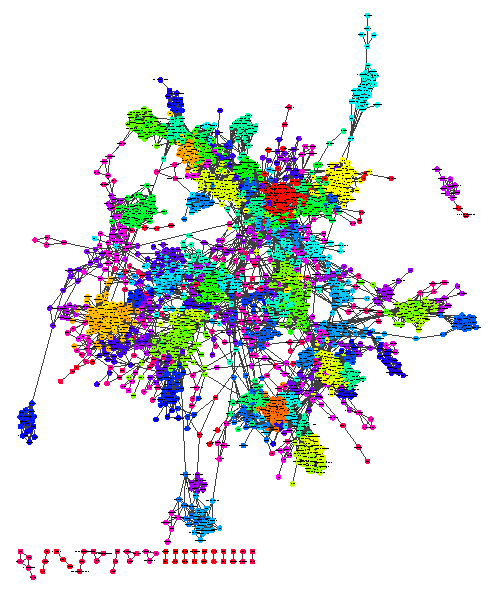
\includegraphics[width=\textwidth]{openimage-communities}
	\caption{The concepts uncovered by using the OpenImages data as input to our algorithm.
	The labels are legible through zooming in the electronic version. See Figure \ref{fig:openimage-zoom} for zoomed-in crops of the graph.}
	\label{fig:openimages-concepts}
\end{figure}


\begin{figure}
	\centering
	\begin{subfigure}{\textwidth}
		\centering
		
\includegraphics[height=0.44\textheight]{openimage-communities-military}
		\caption{A concept that brings together uniformed people and military objects.}
		\label{fig:openimages-military}
	\end{subfigure}
	 %add desired spacing between images, e. g. ~, \quad, \qquad, \hfill etc.
	%(or a blank line to force the subfigure onto a new line)
	\begin{subfigure}{\textwidth}
		\centering
		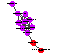
\includegraphics[height=0.44\textheight]{openimage-communities-cameras}
		\caption{A concept that groups together camera equipment.}
		\label{fig:openimages-cameras}
	\end{subfigure}
	\caption{Two visual concepts from the top-right corner of
		Figure \ref{fig:openimages-concepts}.}
	\label{fig:openimage-zoom}
\end{figure}

\subsection{Word similarity evaluation}

To provide a quantitative evaluation of the method we made use of the WordSim-353 (WS-353)
dataset. This dataset includes 353 word pairs that are rated by humans for their
similarity. This dataset includes unrelated words which presents a problem for
our approach that by design does not calculate similarities for words that are unrelated,
as using the graph structure is one of the main ways we can make the computation
scale. For that reason we use the word pairs that appear both in the evaluation
dataset \textit{and} exist in our similarity graph. We use the Google n-grams
data with a corpus of 361 billion tokens, which in under 10 minutes produces
a similarity graph that contains 60\% of the word pairs present in WS-353.

The produced similarities have a Spearman rank correlation of 0.76, which
is exactly what the inter-annotator agreement is for this dataset.
Finally we compare the WS-353 and our produced similarities with the
cosine similarities of the GloVe~\cite{glove} embedding vectors,
which was at the time of publication the state of the art language embedding
method. We train our method on a smaller corpus and smaller window than
the GloVe vectors, but are still able to generate similarities comparable
to GloVe (0.71 Spearman rank correlation).

\section{Discussion}
\label{sec:concepts-discussion}

In this chapter we presented our work on scalable vertex similarity and concept
discovery. We made use of approximations to dramatically reduce the amount of
computation, first by using locality in our computations, and then by taking
advantage of the structure of the graphs to dramatically reduce the number of
edges that are involved in our similarity calculations, further decreasing the
computational cost. We designed the algorithm for a distributed setting, and
through careful design of the similarity calculation step, we are able to minimize
the amount of network communication necessary. Thus, in this work we cover
two of the three objectives defined in Section \ref{sec:intro-question-objectives}
and tackle our original research question in the context of vertex similarity.